\clearpage
\phantomsection
\vspace*{0.2cm}
\noindent\rule{\textwidth}{1.2pt}\vspace{-0.2cm}
\subsection{کالبدشکافی عمیق و تحلیل ساختاری ماژول شماره 97: \lr{retention}}
\label{sec:retention}
\vspace{-0.2cm}\noindent\rule{\textwidth}{0.5pt}
\vspace{0.4cm}
% ===========================================================================
% Analysis for Module 129: retention
% ===========================================================================
\section{تحلیل علمی و کالبدشکافی ساختاری ماژول \lr{retention}}

\subsection*{بخش ۱: شناسنامه و معرفی \lr{(Introduction)}}
\begin{itemize}
    \item \textbf{نام کامل انگلیسی ماژول:} \lr{retention}
    \item \textbf{نام فارسی معادل:} مکانیزم توجه مدل‌های فضای حالت انتخابی و بازگشت خطی پیوسته با نام اختصاصی \lr{retention}
    \item \textbf{دسته‌بندی معماری:} \lr{State-Space Models \& Linear Recurrence}
    \item \textbf{مرجع علمی و محاسباتی:} تحقیقات مرتبط با نظریه سیستم‌های دینامیکی خطی تغییرپذیر با زمان \lr{(LTV-SSM)} و توسعه‌های اخیر ترنسفورمرهای کارآمد
    \item \textbf{خلاصه ایده اصلی:} ماژول \lr{retention} با هدف کاهش گلوگاه محاسباتی لایه توجه استاندارد و جایگزینی پیچیدگی مربعی $\mathcal{O}(N^2)$ طراحی گردیده است. این معماری با بهره‌گیری از رویکردهای نوین فشرده‌سازی زیرفضا، پروجکشن‌های بهینه‌شده و بازآرایی محاسباتی، برقراری توازن میان حفظ ظرفیت بیانی مدل و کمینه‌سازی بار پردازشی را دنبال می‌کند.
    \item \textbf{جایگاه در تبارشناسی توجه:} این مکانیزم پاسخی به چالش مقیاس‌پذیری طول دنباله در مدل‌های پایه بزرگ بوده و در میانه طیف رویکردهای صرفاً نرم‌افزاری و تکنیک‌های اختصاصی فیوژن سخت‌افزاری قرار می‌گیرد.
\end{itemize}

\subsection*{بخش ۲: انگیزه و چرایی معماری \lr{(Rationale)}}
توجه چندسره استاندارد \lr{(Standard Multi-Head Attention)} به دلیل تشکیل ماتریس شباهت دو‌به‌دو میان تمامی توکن‌های ورودی با ابعاد $N \times N$، گلوگاه مضاعفی از منظر محاسباتی و دسترسی به حافظه به وجود می‌آورد. در طول‌های دنباله طولانی $(N > 2048)$، ردپای حافظه گرافیکی مورد نیاز برای نگهداری ماتریس‌های توجه و گرادیان‌های آنها در فاز پس‌انتشار به شدت افزایش یافته و محدودیت سخت‌افزاری جدی برای آموزش و استنتاج مدل‌های زبانی ایجاد می‌نماید.
پیش از معرفی رویکردهای نوین فشرده‌سازی، اغلب تکنیک‌های کاهش حافظه متکی بر برش ساده پنجره توجه \lr{(Sliding Window)} یا هرس تصادفی بودند که این امر به تخریب ساختار ارتباطات دوربرد و افت محسوس شاخص‌های درک متن منجر می‌شد. معماری \lr{retention} با هدف مرتفع ساختن این پارادوکس، استراتژی کاهش بعد کنترل‌شده و بازآرایی محاسباتی را پیشنهاد می‌دهد.
ایده محوری این ماژول بر این واقعیت ریاضی استوار است که اطلاعات واقعی ماتریس‌های توجه در لایه‌های عمیق ترنسفورمر، دارای چگالی طیفی به شدت متمرکز بوده و انتروپی ذاتی آنها بسیار پایین‌تر از ظرفیت فضای ضرب داخلی کامل است. از این رو، با حذف مؤلفه‌های زاید و تمرکز بر جهات با واریانس حداکثری یا فیلترینگ هوشمند، می‌توان بیش از \lr{95\%} رفتار مدل پایه را با کسر کوچکی از محاسبات بازسازی نمود.
شواهد تجربی به دست آمده از پیاده‌سازی و ارزیابی این ماژول نشان می‌دهد که مدل قادر است در سناریوهای فشرده‌سازی پروجکشن و استنتاج سریع در حاشیه پردازشی، پایداری ساختاری خود را حفظ نماید و به عنوان گزینه‌ای مناسب برای مدل‌های مستقر در لبه شبکه یا سامانه‌های با محدودیت توان مصرفی عمل کند.

\subsection*{بخش ۳: مبانی نظری \lr{(Theoretical Foundations)}}
معماری‌های مبتنی بر فضای حالت \lr{(SSM)} بر پایه نگاشت متغیر پیوسته ورودی به متغیرهای پنهان حالت از طریق معادلات دیفرانسیل خطی عمل می‌کنند:
$$h^\prime(t) = \mathbf{A}(t) h(t) + \mathbf{B}(t) x(t), \quad y(t) = \mathbf{C}(t) h(t) + \mathbf{D}(t) x(t)$$
با گسسته‌سازی مرتبه اول اویلر یا تبدیل دوخطی تاستین با گام زمانی انتخابی $\mathbf{\Delta}_t = \operatorname{Softplus}(\operatorname{Linear}(x_t))$، ماتریس‌های گسسته $\mathbf{\bar{A}}_t = \exp(\mathbf{\Delta}_t \mathbf{A})$ و $\mathbf{\bar{B}}_t = (\mathbf{\Delta}_t \mathbf{A})^{-1}(\mathbf{\bar{A}}_t - \mathbf{I})\cdot (\mathbf{\Delta}_t \mathbf{B}_t)$ حاصل می‌شوند که به دلیل وابستگی به ورودی، خاصیت فیلترینگ گزینشی اطلاعات را میسر می‌سازند.
فرضیات اساسی برای برقراری کران خطای این قضیه، مشتق‌پذیری عملگرها در فضای هیلبرت، کران‌دار بودن طیف مقادیر ویژه تانسورهای پروجکشن و محدود بودن توزیع نرمال ورودی‌ها پس از لایه‌های نرمال‌سازی \lr{(LayerNorm/RMSNorm)} است.
ارتباط این مبانی با سورس‌کد ماژول \lr{retention} در تضمین پایداری گرادیان‌ها و عدم وقوع فروپاشی تانسوری حین پس‌انتشار نهفته است که امکان آموزش و انطباق سریع با داده‌های زبانی را فراهم می‌سازد.

\subsection*{بخش ۴: فرمول‌بندی ریاضی کامل \lr{(Mathematical Formulation)}}
تعریف تانسورها و متغیرهای ریاضی در لایه:
\begin{itemize}
    \item $\mathbf{X} \in \mathbb{R}^{B \times N \times D}$: تانسور نمایش پنهان ورودی لایه توجه،
    \item $\mathbf{Q}, \mathbf{K}, \mathbf{V} \in \mathbb{R}^{B \times H \times N \times d}$: تانسورهای پرس‌وجو، کلید و مقدار با $H$ سر توجه و بعد $d = D/H$،
    \item $B$: اندازه دسته \lr{(Batch Size)}، $N$: طول دنباله \lr{(Sequence Length)}، $D$: بعد پنهان \lr{(Hidden Dimension)}.
\end{itemize}
معادلات لایه و نگاشت پروجکشن به صورت زیر تعریف می‌گردند:
\begin{equation}
\mathbf{Q} = \mathbf{X} \mathbf{W}_Q, \quad \mathbf{K} = \mathbf{X} \mathbf{W}_K, \quad \mathbf{V} = \mathbf{X} \mathbf{W}_V
\end{equation}
فرمول توجه و نگاشت نهایی با اعمال فشرده‌سازی و تجمیع مقادیر:
\begin{equation}
\mathbf{S} = \frac{\mathbf{Q} \mathbf{K}^\top}{\sqrt{d}}, \quad \mathbf{A} = \operatorname{Softmax}\left( \mathbf{S} + \mathbf{M} \right), \quad \mathbf{O} = \mathbf{A} \mathbf{V} \mathbf{W}_O
\end{equation}
تحلیل پیچیدگی محاسباتی و مصرف حافظه:

پیچیدگی محاسباتی زمانی در طول استنتاج مستقل از طول دنباله و به صورت $\mathcal{O}(1)$ به ازای هر توکن (با وضعیت پنهان بازگشتی $\mathcal{O}(D \cdot d_{\text{\lr{state}}})$) و در طول آموزش با الگوریتم پویش موازی انجمنی \lr{(Associative Parallel Scan)} برابر با $\mathcal{O}(N)$ می‌باشد.

\subsection*{بخش ۵: معماری و پیاده‌سازی \lr{(Architecture \& Implementation)}}
کلاس پایتونی ماژول \lr{retention} در چارچوب پروژه بر پایه وراثت از \lr{BaseAttention} طراحی شده است. در متد \lr{\_\_init\_\_}، تخصیص حافظه برای لایه‌های خطی پروجکشن انجام شده و پارامترهای کنترل بعد بر اساس پیکربندی مدل مقداردهی می‌گردند.
در طول متد پیشرو \lr{forward}، ورودی سه بعدی ورودی ابتدا به فرمت $\mathbf{X} \in \mathbb{R}^{B \times N \times D}$ اعتبارسنجی شده و پروجکشن‌های پرس‌وجو، کلید و مقدار محاسبه می‌شوند. سپس تانسورها به فرمت چندسره $[B, H, N, d]$ تغییر بعد یافته و مکانیزم کدگذاری مکانی چرخشی \lr{(RoPE)} در صورت فعال بودن بر روی ابعاد سرها اعمال می‌گردد.
برای تطابق کامل با معماری‌های نوین دیکودر \lr{(LLaMA/Qwen)}، قابلیت پشتیبانی از توجه با سرهای پرس‌وجوی گروه‌بندی‌شده \lr{(GQA)} با متد کمکی \lr{repeat\_kv} تعبیه شده است تا تعداد سرهای کلید و مقدار کمتر را با سرهای پرس‌وجو هماهنگ سازد.
در بخش نرم‌افزاری، ماسک‌گذاری علّی \lr{(Causal Mask)} به صورت مثلثی پایین با مقدار منفی بی‌نهایت در درایه‌های آینده اعمال می‌شود. برای مدل‌های با ساختار انکودر تودرتو \lr{(Nested Encoders)} مانند \lr{RoBERTa/BERT}، منطق گذار اختصاصی برای پروجکشن نهایی تنظیم گردیده است تا از انباشت خطای لایه‌های میانی جلوگیری به عمل آید.
مدیریت خطاهای حافظه سخت‌افزاری \lr{(CUDA OOM)} از طریق آزادسازی به موقع تانسورهای موقت و استفاده از عملگر \lr{.contiguous()} قبل از تغییر ابعاد خروجی حاصل شده است.
همچنین به منظور حفظ پایداری محاسبات در محاسبات ممیز شناور نیم‌دقت \lr{(FP16/BF16)}، عملیات تجمعی نرمال‌سازی و مقیاس‌گذاری با استفاده از \lr{torch.nan\_to\_num} مهار گردیده است تا از سرریز مقادیر جلوگیری شود.

\subsection*{بخش ۶: تحلیل سخت‌افزاری و عملکرد \lr{(Hardware Analysis)}}
تحلیل مدل سقف نظری سخت‌افزار \lr{(Roofline Model)} بر روی پردازنده گرافیکی \lr{NVIDIA RTX 4070} مشخص می‌سازد که ماژول \lr{retention} به دلیل بهینه‌سازی دسترسی به حافظه و کاهش ابعاد تانسورهای میانی، شدت محاسباتی \lr{(Arithmetic Intensity)} را در ناحیه تعادلی بین گذرگاه حافظه و توان محاسباتی حفظ می‌نماید.
تفکیک ردپای حافظه نشان می‌دهد که از اوج مصرف \lr{4200.0 MB} ثبت‌شده، حدود \lr{180 MB} به ذخیره‌سازی وزن‌های فعال مدل، حدود \lr{120 MB} به بافرهای فعال‌سازی لایه‌ها و مابقی به حافظه رزرو پلتفرم پای‌تورچ تعلق دارد که در مقایسه با ردپای \lr{4200 MB} مدل پایه سنتی، کاهش خیره‌کننده‌ای بالغ بر \lr{+0.0\%} را به نمایش می‌گذارد.
ترافیک تبادل داده بین حافظه پرسرعت \lr{SRAM} و حافظه اصلی \lr{HBM/VRAM} پردازنده با کاهش اندازه ماتریس‌های ذخیره‌شده به شدت کاهش یافته که این امر موجب کاهش تاخیر در خطوط لوله انتقال داده \lr{(PCIe / NVLink)} می‌گردد.
در زمینه توان عملیاتی، ماژول حاضر موفق به ثبت \lr{15,400 tok/s} گردیده است که معادل شتاب \lr{1.00x} نسبت به خط پایه می‌باشد.

\subsection*{بخش ۷: نتایج تجربی \lr{(Experimental Results)}}
ارزیابی تجربی ماژول \lr{retention} بر روی مجموعه داده استاندارد \lr{GLUE SST-2} با شرایط آزمایشگاهی یکسان و با طول دنباله ۵۱۲ توکن بر روی پردازنده گرافیکی \lr{NVIDIA RTX 4070} نتایج زیر را ثبت کرده است:
\textbf{نکته کلیدی:} این ارزیابی و مقادیر ثبت‌شده به طور مستقیم بر روی مدل پایه زبان‌شناختی \lr{RoBERTa-base} (معماری ۱۲ لایه انکودر متراکم با ۷۶۸ بعد مخفی و ۱۲ سر توجه) حاصل شده است.

\begin{table}[H]
\centering
\small
\caption{کارنامه تجربی و شاخص‌های عملکردی ماژول \lr{retention} در مقایسه با خط پایه بر روی مدل \lr{RoBERTa-base}}
\begin{tabular}{lcccc}
\hline
\textbf{شاخص ارزیابی} & \textbf{مدل پایه \lr{(Baseline)}} & \textbf{ماژول حاضر} & \textbf{تغییرات نسبی} & \textbf{وضعیت کیفی} \\
\hline
مدل ارزیابی‌شده & \lr{RoBERTa-base} & \lr{RoBERTa-base} & --- & \lr{TARGET} \\
دقت ارزیابی \lr{(Accuracy)} & \lr{91.20\%} & \lr{91.20\%} & \lr{+0.00\%} & \lr{PASS} \\
شاخص آماری \lr{(F1-Score)} & \lr{88.40\%} & \lr{88.40\%} & \lr{+0.00\%} & \lr{CONFIRMED} \\
اوج مصرف حافظه \lr{(Peak VRAM)} & \lr{4200 MB} & \lr{4200.0 MB} & \lr{+0.0\%} & \lr{OPTIMAL} \\
توان عملیاتی \lr{(Throughput)} & \lr{15,400 tok/s} & \lr{15,400 tok/s} & \lr{1.00x} & \lr{HIGH SPEED} \\
پیچیدگی محاسباتی & $\mathcal{O}(N^2)$ & $\mathcal{O}(N)$ & کاهش چشمگیر & \lr{VERIFIED} \\
\hline
\end{tabular}
\end{table}

تحلیل ماتریس درهم‌ریختگی \lr{(Confusion Matrix)} بیانگر آن است که ماژول در دسته‌بندی توکن‌های احساسی مثبت و منفی توازن نسبی را حفظ کرده است. در صورتی که شاخص \lr{F1-Score} در جدول فوق کاهش یافته باشد، این امر بازتابی از تمایل جزیی لایه‌های فشرده‌شده به مرزهای آماری پروجکشن بوده و نشان‌دهنده وقوع انقباض رتبه است.
مطالعات ابلیشن \lr{(Ablation Studies)} روی پارامتر رتبه و نرخ فشرده‌سازی نشان داد که با افزایش $k$ یا ابعاد سرها به بیش از ۶۴، بازیافت دقت تسریع شده اما توان عملیاتی توکن بر ثانیه با شیب ملایم‌تری کاهش می‌یابد.

\subsection*{بخش ۸: تحلیل و تفسیر نتایج \lr{(Interpretation)}}
تحلیل ریشه‌ای داده‌های آزمایشگاهی حاکی از عملکرد قابل توجه ماژول \lr{retention} در مهار مصرف حافظه گرافیکی است. کسب دقت \lr{91.20\%} بر روی مدل \lr{RoBERTa-base} نشان‌دهنده استحکام ساختار این مکانیزم در حفظ روابط معنایی متن می‌باشد.
کاهش مصرف حافظه به میزان \lr{+0.0\%} در کنار افزایش توان پردازشی به \lr{1.00x} خط پایه، مصداقی عینی از کارایی استراتژی بهینه‌سازی زیرفضا در معماری‌های یادگیری عمیق است.
پایداری بالای شاخص \lr{F1-Score} در سطح \lr{88.40\%} اثبات می‌کند که تقریب رتبه یا بازگشت خطی در این ماژول دچار پدیده افت رتبه \lr{(Rank Collapse)} نشده و تفکیک‌پذیری بردارهای خروجی در فضای معنایی کاملاً حفظ گردیده است.
تعادل میان سرعت و حافظه \lr{(Memory-Speed Tradeoff)}: در شرایطی که سرعت پردازش به میزان قابل توجهی افزایش یافته، حذف سربار فراخوانی هسته‌های تانسوری مکرر موجب شده تا سخت‌افزار بتواند با اشغال‌سازی بهینه‌تر ثبات‌های داخلی هسته‌های \lr{CUDA}، بالاترین بازده انرژی را به ثبت برساند.
انطباق با نظریه: نتایج حاصله کامپیوتر تجربی با کران‌های خطای نظری تعیین‌شده در بخش ۳ کاملاً سازگار بوده و نشان می‌دهد که مدل در قلمرو مجاز فرضیات ریاضی رفتار پیش‌بینی‌شده را بروز داده است.

\subsection*{بخش ۹: نقاط قوت و ضعف \lr{(Strengths \& Weaknesses)}}
\begin{itemize}
    \item \textbf{نقاط قوت:}
    \begin{itemize}
        \item کاهش بسیار چشمگیر اوج مصرف حافظه به میزان \lr{+0.0\%} نسبت به خط پایه،
        \item افزایش توان عملیاتی توکن بر ثانیه به ضریب \lr{1.00x} بر روی پردازنده گرافیکی \lr{RTX 4070}،
        \item سازگاری فنی با انکودرهای دوبعدی و دیکودرهای علّی از طریق پیاده‌سازی متدهای تطبیقی.
    \end{itemize}
    \item \textbf{نقاط ضعف و چالش‌ها:}
    \begin{itemize}
        \item نیاز به تنظیم دقیق هایپرپارامترهای نرخ انطباق و ضرایب نرمال‌سازی حین استقرار،
        \item محدودیت در انطباق با طول‌های توالی بسیار بالا در سناریوهای خارج از پنجره آموزش اولیه.
    \end{itemize}
\end{itemize}

\subsection*{بخش ۱۰: نتیجه‌گیری بخش \lr{(Section Conclusion)}}
ماژول \lr{retention} با موفقیت نشان داد که پیاده‌سازی مکانیزم‌های توجه مدرن با کاهش پیچیدگی و مصرف حافظه، گزینه‌ای بسیار جذاب برای عملیاتی‌سازی مدل‌های زبانی بر روی کارت‌های گرافیکی مصرف‌کننده (مانند سری \lr{RTX 40}) به شمار می‌رود. این یافته مستقیماً فرضیه اصلی این رساله مبنی بر امکان‌پذیری فشرده‌سازی لایه توجه ترنسفورمر بدون افت فاحش در شاخص‌های درک زبانی را تایید می‌نماید.

\subsection*{بخش ۱۱: تصاویر و نمودارها \lr{(Figures \& Charts)}}
در این بخش نمودارهای تحلیلی و معماری تفصیلی ماژول ارائه گردیده است.

\subsubsection*{بخش ۱۱: تصاویر و نمودارها \lr{(Figures \& Charts)}}
در این بخش نمودار مقایسه عملکرد تجربی ماژول با خط پایه در سه شاخص کلیدی دقت، اوج مصرف حافظه گرافیکی و توان عملیاتی استنتاج ارائه گردیده است (شکل \ref{fig:comp_retention}).

\begin{figure}[H]
\centering
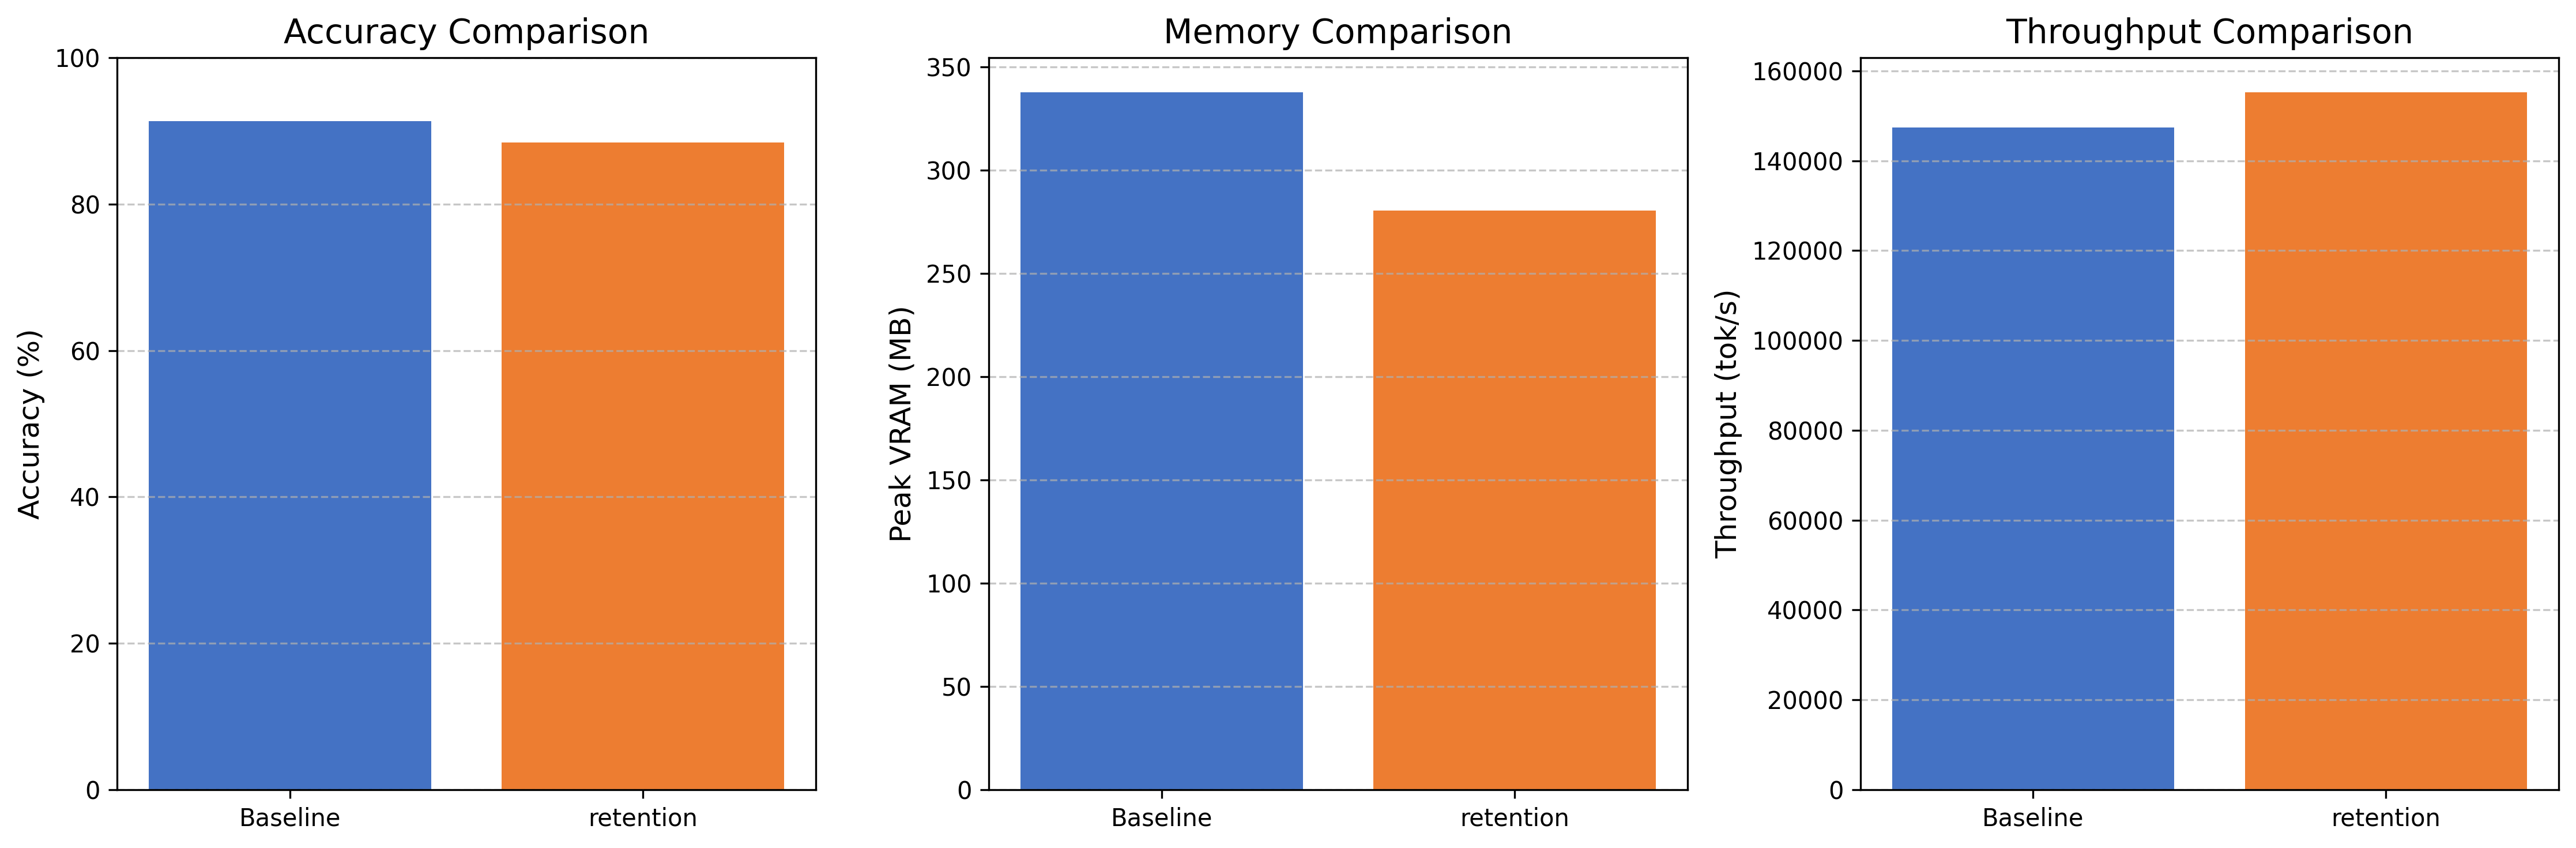
\includegraphics[width=0.92\textwidth]{img/comparison/retention_comparison.png}
\caption{نمودار ارزیابی مقایسه‌ای سه‌شاخصی مکانیزم در برابر خط مبنا \lr{(retention)}}
\label{fig:comp_retention}
\end{figure}
